\documentclass{beamer}
\usepackage{amsmath,amstext,amsfonts,amssymb} %Mathe-Formeln
\graphicspath{{images/}}
%PDF-Dokumente einbinden
\usepackage{epstopdf}
\usepackage{pdfpages}
\usepackage{subfig}
\usepackage{tikz}
\usetikzlibrary{shapes,arrows,automata,matrix,trees}
\usetikzlibrary{decorations.pathreplacing,calc,positioning}
\usetikzlibrary{fit}					% fitting shapes to coordinates
\usetikzlibrary{dsp,chains}
\usepackage{tikz-timing}[2009/12/09]
\usetikztiminglibrary[new={char=Q,reset char=R}]{counters}
\usetikzlibrary{decorations,arrows} 
\usetikzlibrary{decorations.pathmorphing} 
\usepgflibrary{decorations.pathreplacing} 
\usetikzlibrary{dsp,chains}
\usepackage{caption}

%Anzeige mathematischer Symbole
\usepackage{amssymb}
%Anzeige von mathematischer Umgebung
\usepackage{amsthm}
\usepackage{stmaryrd}
\usepackage{verbatim}


\usepackage[utf8]{inputenc}
\usepackage[ngerman]{babel}
\usepackage{pgf}
\usepackage[OT1]{fontenc} % Ligaturen, richtige Umlaute im PDF
%Umschalten der Sprache
\selectlanguage{ngerman}
\newcommand{\fullname}{Andreas Rehn}
\newcommand{\titel}{Entwicklung einer Dopplerinstrumentierung zur Detektion von Luftembolien in einem künstlichen Blutkreislauf}
%was ist definiert

\usetheme{Dresden}
\beamertemplatenavigationsymbolsempty
%\setbeamercovered{transparent}
\usepackage{bbding}
\newcommand*\tick{\item[\Checkmark]}
\newcommand*\fail{\item[\XSolidBrush]}

\tikzset{%
  block/.style    = {draw, , rectangle, minimum height = 3em,
    minimum width = 3em},
  sum/.style      = {draw, circle, node distance = 2cm}, % Adder
  input/.style    = {coordinate}, % Input
  output/.style   = {coordinate}, % Output
  right iso/.style={isosceles triangle,scale=0.5,sharp corners, anchor=center, xshift=-4mm},
  left iso/.style ={right iso, rotate=180, xshift=-8mm},
  txt/.style	  ={text width=1.5cm,anchor=center},
  ellip/.style	  ={ellipse,scale=0.5},
  empty/.style	  ={draw=none}
}

\tikzstyle{block} = [draw, rectangle, 
    minimum height=3em, minimum width=6em]
\tikzstyle{sum} = [draw, fill=blue!20, circle, node distance=2cm]
\tikzstyle{input} = [coordinate]
\tikzstyle{output} = [coordinate]
\tikzstyle{pinstyle} = [pin edge={to-,thin,black}]

\usepackage{pgfplots}
\pgfplotsset{width=7cm,compat=1.8}

%
%
%
%
\newcommand*\annotatedFigureBoxCustom[8]{\draw[#5,line width=0.75mm,rounded corners] (#1) rectangle (#2);\node at (#4) [fill=#6,thick,shape=circle,draw=#7,inner sep=2pt,font=\sffamily,text=#8] {\textbf{#3}};}
%\annotatedFigureBox{bottom-left}{top-right}{label}{label-position}
\newcommand*\annotatedFigureBox[4]{\annotatedFigureBoxCustom{#1}{#2}{#3}{#4}{black}{black}{white}{white}}
\newcommand*\annotatedFigureText[4]{\node[draw=none, anchor=south west, text=#2, inner sep=0, text width=#3\linewidth,font=\sffamily] at (#1){#4};}
\newenvironment {annotatedFigure}[1]{\centering\begin{tikzpicture}
\node[anchor=south west,inner sep=0] (image) at (0,0) { #1};\begin{scope}[x={(image.south east)},y={(image.north west)}]}{\end{scope}\end{tikzpicture}}
%%%%%%%%%%%%%%%%%%%%%%%%%%%%%%%%%%%%%%%%%%%%%%%%%%%%%%%%%%%%%%%%%%%%%%
%
%
%
%

\begin{document}

\title{\titel}
\author[A. Rehn]{\fullname}
\institute[IMM - HS Ulm]{Fakultät Mechatronik und Medizintechnik\\ Hochschule Ulm}
\titlegraphic{
\includegraphics[width=0.14\textwidth]{logo}}
\date[04.11.15]{04. November 2015}

\frame{\titlepage}

\expandafter\def\expandafter\insertshorttitle\expandafter{%
  \insertshorttitle\hfill\insertframenumber}%\,/\,\inserttotalframenumber}

\begin{frame}{über mich}
	\begin{columns}
	\column{.2\textwidth} 
		\begin{figure}[h]
			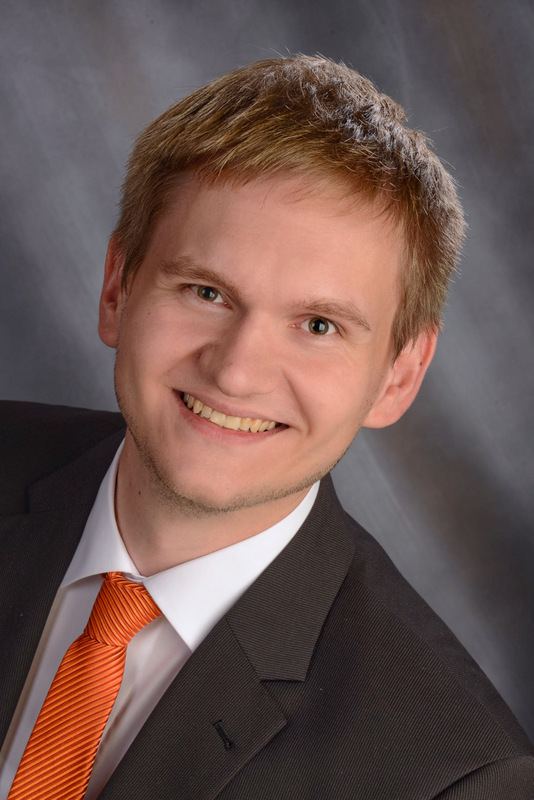
\includegraphics[width=1\textwidth]{images/me}
		\end{figure}
	\column{.6\textwidth}
		\begin{block}{Andreas Rehn}
		\begin{itemize}			
			\item B.Eng Mechatronik
			\item cand. M.Eng. Systems Engineering and Management
		\end{itemize}
		\end{block}
	\end{columns}

\end{frame}
  
\logo{\pgfimage[width=0.1\textwidth]{images/logo}}
%\setbeamertemplate{footline}[frame number]

\frame{\frametitle{Agenda}
	\tableofcontents
	[pausesections]
}

\section{Einleitung}
\subsection{Dedetektion von Embolien mittels Ultraschall}
\begin{frame}{Embolien}
	\begin{columns}
	\column[t]{.38\textwidth}
		\begin{block}{Arten}
			\begin{itemize}
				\item Luft- / Gasembolie
				\item Tromboembolie
				\item Fettembolie
			\end{itemize}
		\end{block}
		\begin{block}{Folgen}
			\begin{itemize}
				\item minderperfundierte Gewebestrukturen
				\item Tod
			\end{itemize}
		\end{block}
	\column[t]{.3\textwidth} 
	\centering
		\begin{figure}[t]
			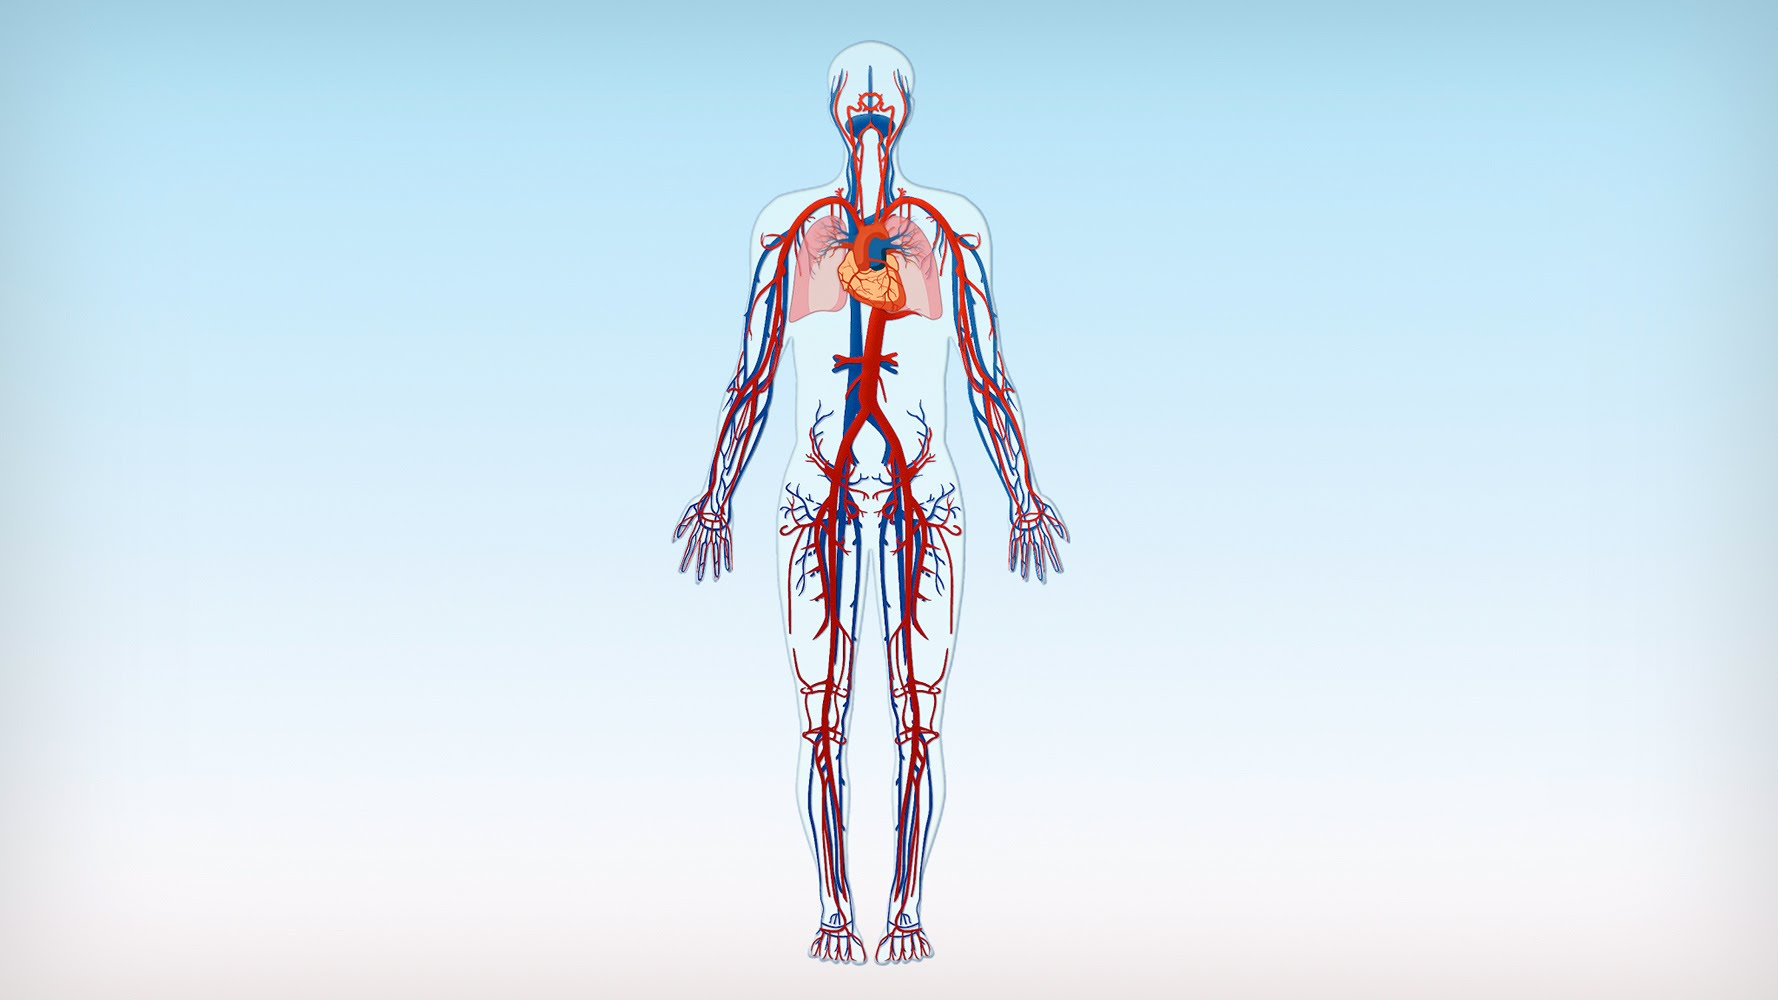
\includegraphics[trim = 24cm 1cm 25cm 1cm, clip=true, width=1\textwidth]{Praesentation/maxresdefault}
%			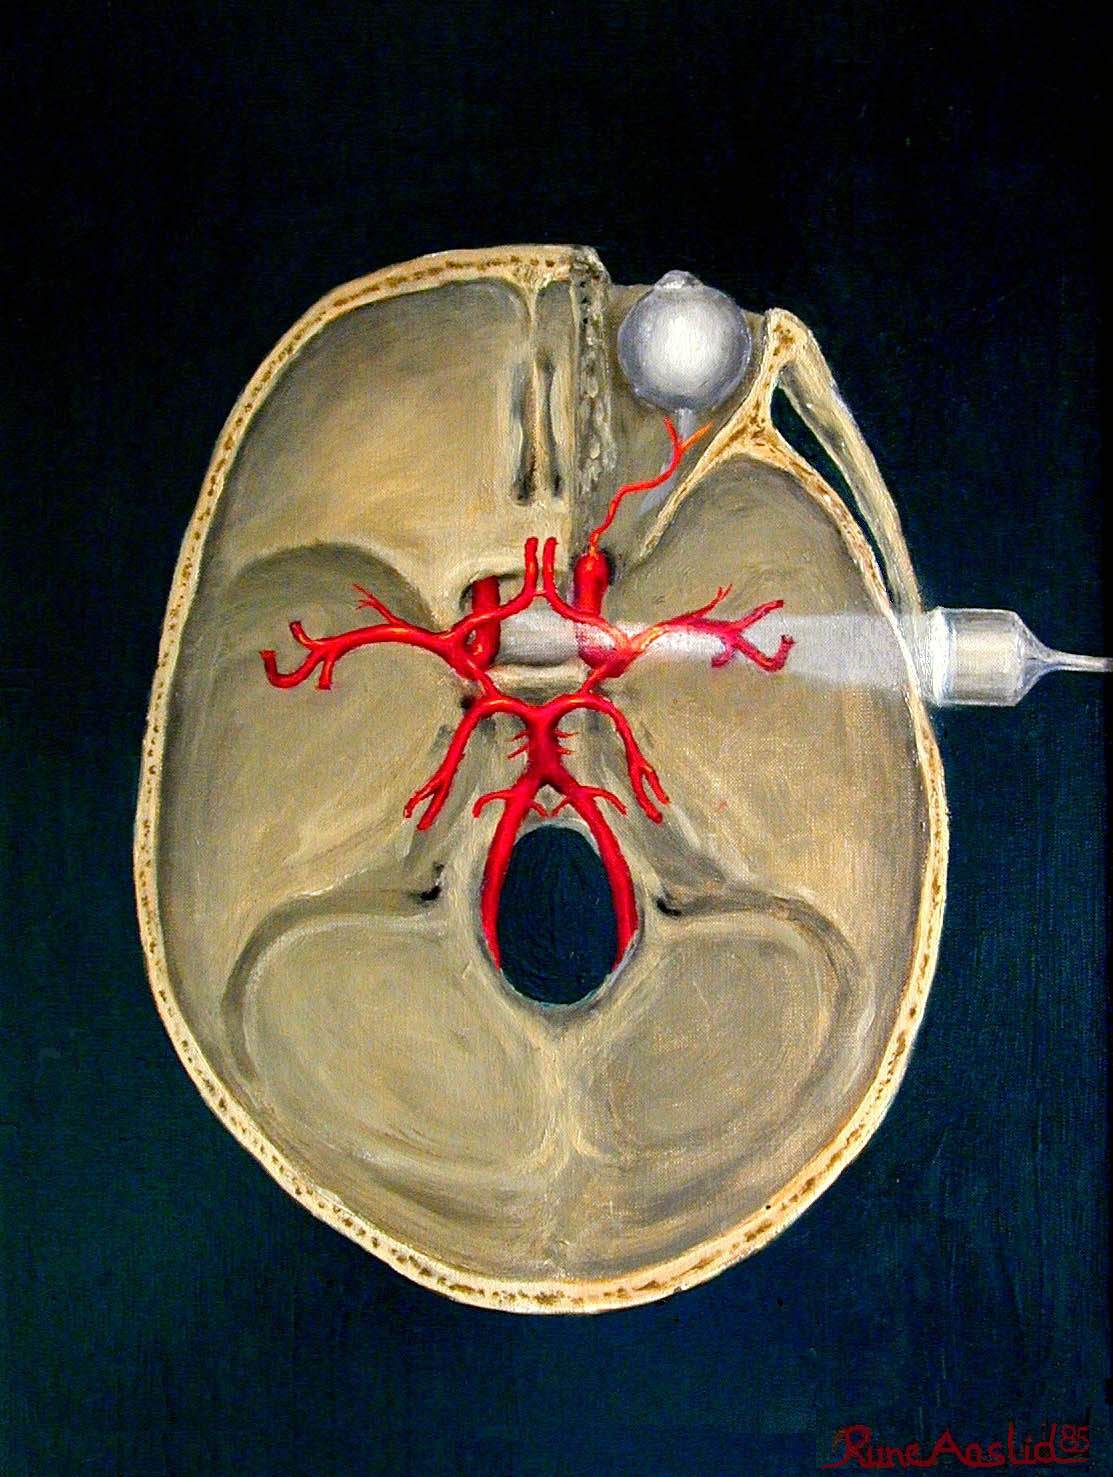
\includegraphics[width=1\textwidth]{Praesentation/Transcranial_doppler}
			%https://upload.wikimedia.org/wikipedia/en/7/7c/Transcranial_doppler.jpg
			%http://i.ytimg.com/vi/Jp1URHU7arY/maxresdefault.jpg
		\end{figure}
	\end{columns}
\end{frame}
%
%
%
%
%
\begin{frame}
\begin{columns}
	\column{.4\textwidth} 
		\begin{figure}[h]
			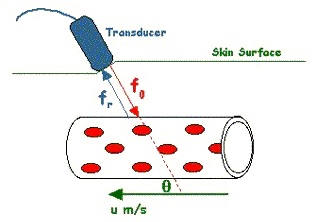
\includegraphics[width=1\textwidth]{pw/DopplerBloodFlow}
		\end{figure}
	\column{.6\textwidth}
		\begin{block}{Strömungsprofilermittlung basierend auf Doppereffekt}
		\begin{itemize}
			\item $\Delta f= f_0-f= \dfrac{2f_0\cdot cos\left(\theta\right)}{\upsilon}$
			\item[\Checkmark] $\upsilon=\dfrac{2f_0\cdot cos\left(\theta\right)}{\Delta f}$
		\end{itemize}
		\end{block}
\end{columns}
\end{frame}

\begin{frame}{Strömungsprofile}
\begin{columns}
	\column{.48\textwidth} 
		\begin{figure}[h]
			\includegraphics[page=2,trim = 45mm 77mm 140mm 45mm, clip=true,width=0.9\textwidth]{vortrag/Vortrag.pdf}
			\caption{Beispiel Arteria femoralis}
		\end{figure}
	\column{.48\textwidth}
		\begin{figure}[h]
			\includegraphics[page=2,trim = 120mm 77mm 60mm 45mm, clip=true,width=0.9\textwidth]{vortrag/Vortrag.pdf}
			\caption{Beispiel Arteria carotis communis}
		\end{figure}
\end{columns}
\end{frame}

\begin{frame}{Strömungsprofil als Spektrogramm}
\begin{figure}[h]
			\includegraphics[page=3,trim = 3mm 15mm 10mm 43mm, clip=true,width=0.9\textwidth]{vortrag/Vortrag.pdf}
			\caption{Arteria carotis communis}
		\end{figure}
\end{frame}
%
%
%
%
\subsection{Stand der Technik}
\begin{frame}{pulsed wave Ultrasonic Doppler - analoge Umsetzung I}
\begin{figure}
	\centering
	\includegraphics[page=2,trim = 13mm 60mm 1mm 58mm, clip=true, width=\textwidth]{Ultrasound/pw_rx}
	\caption{Block Diagramm eines analogen PW Doppler Systems}
\label{fig:analog_pwd_bloc}
\end{figure}
\begin{itemize}
			\item[\Checkmark] longitudinale Ausbreitung
			\item[\Checkmark] Frequenzen von 2 bis 8 MHz			
			\item[\Checkmark] variable Energie/ -dichte
			\item[\Checkmark] Gewebetiefen bis 80 mm
		\end{itemize}
\end{frame}
\begin{frame}{pulsed wave Ultrasonic Doppler - analoge Umsetzung II}
\begin{figure}
	\centering
	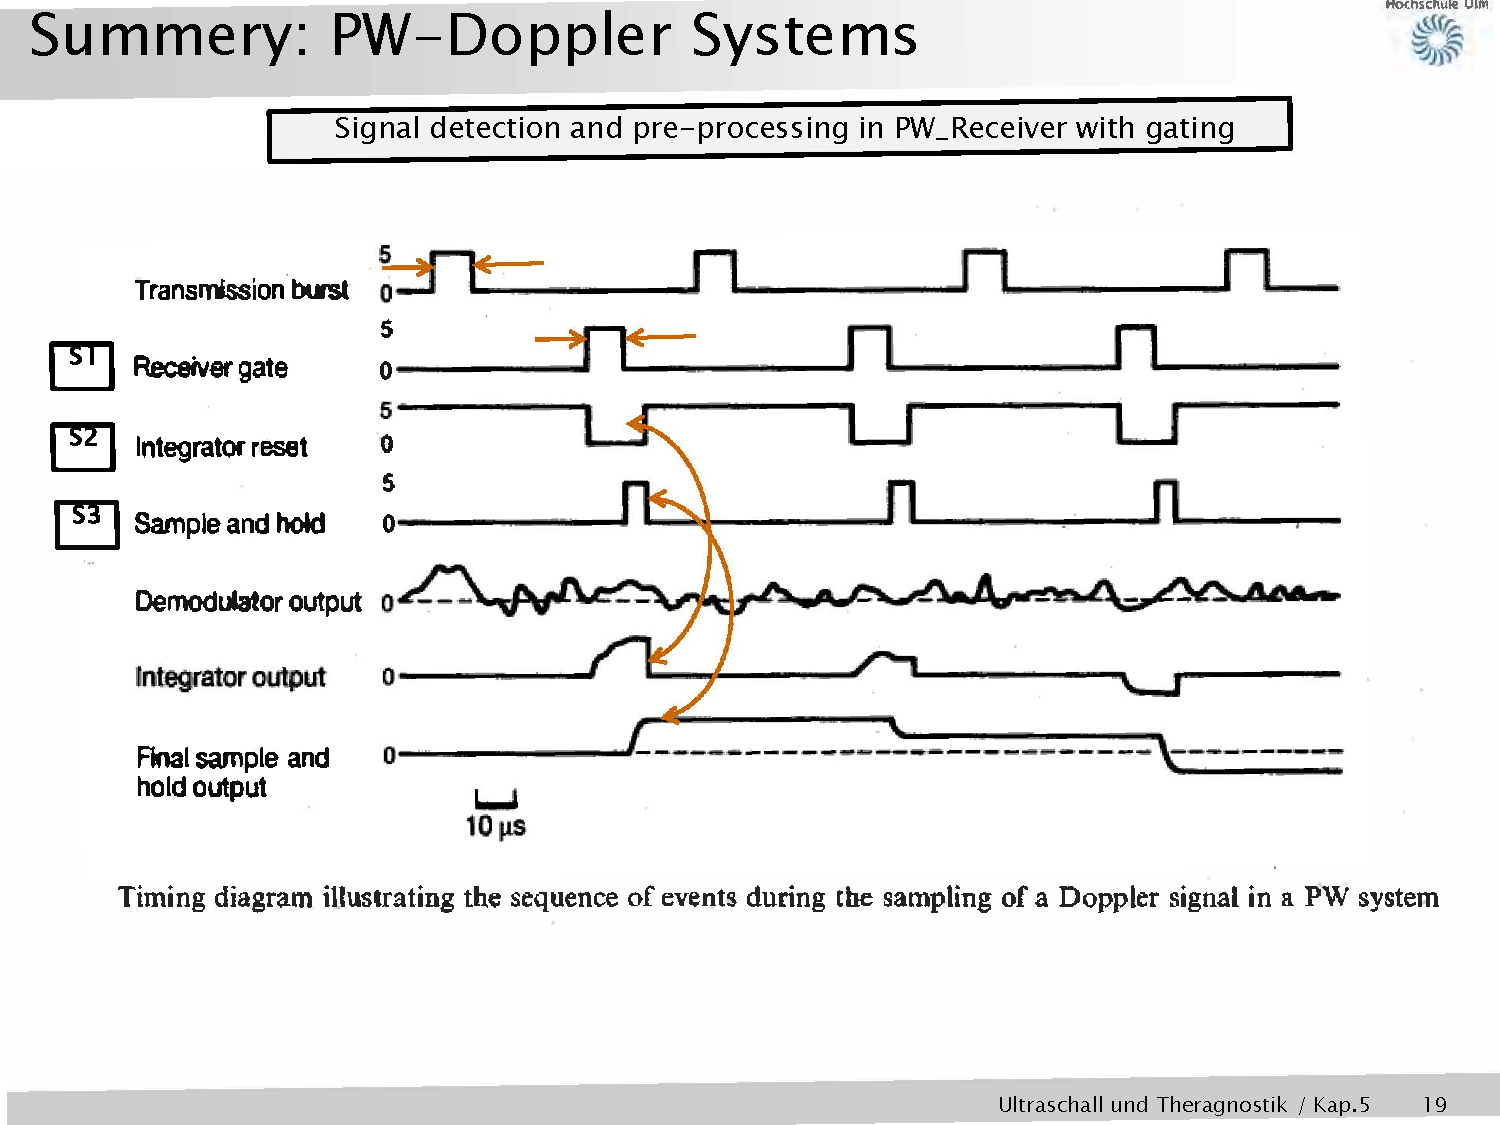
\includegraphics[page=1,trim = 23mm 48mm 27mm 42mm, clip=true, width=0.8\textwidth]{Ultrasound/pw_rx}
	\caption{Ereignis-Zeitdiagramm für die Verarbeitung eines analogen Demodulatorausgangs}
\label{fig:demodulator}
\end{figure}
\end{frame}


\begin{frame}{Visualisierung I}
\begin{columns}
	\column[t]{.7\textwidth}
		\begin{figure}[t]
			\includegraphics[page=3,trim = 80mm 88mm 38mm 52mm, clip=true, width=\textwidth]{Ultrasound/pw_rx}
			\caption{Hüllkurve - Amplitude der I/Q-Signale}
		\end{figure}
	\column[t]{.2\textwidth} 
	\centering
		\begin{figure}[t]
			\includegraphics[trim = 80mm 0mm 0mm 0mm, clip=true, height=3cm,]{Ultrasound/b-Mode}
			\caption{B-Mode}
		\end{figure}
	\end{columns}
\end{frame}

\begin{frame}{Visualisierung II}
\begin{figure}[t]
			  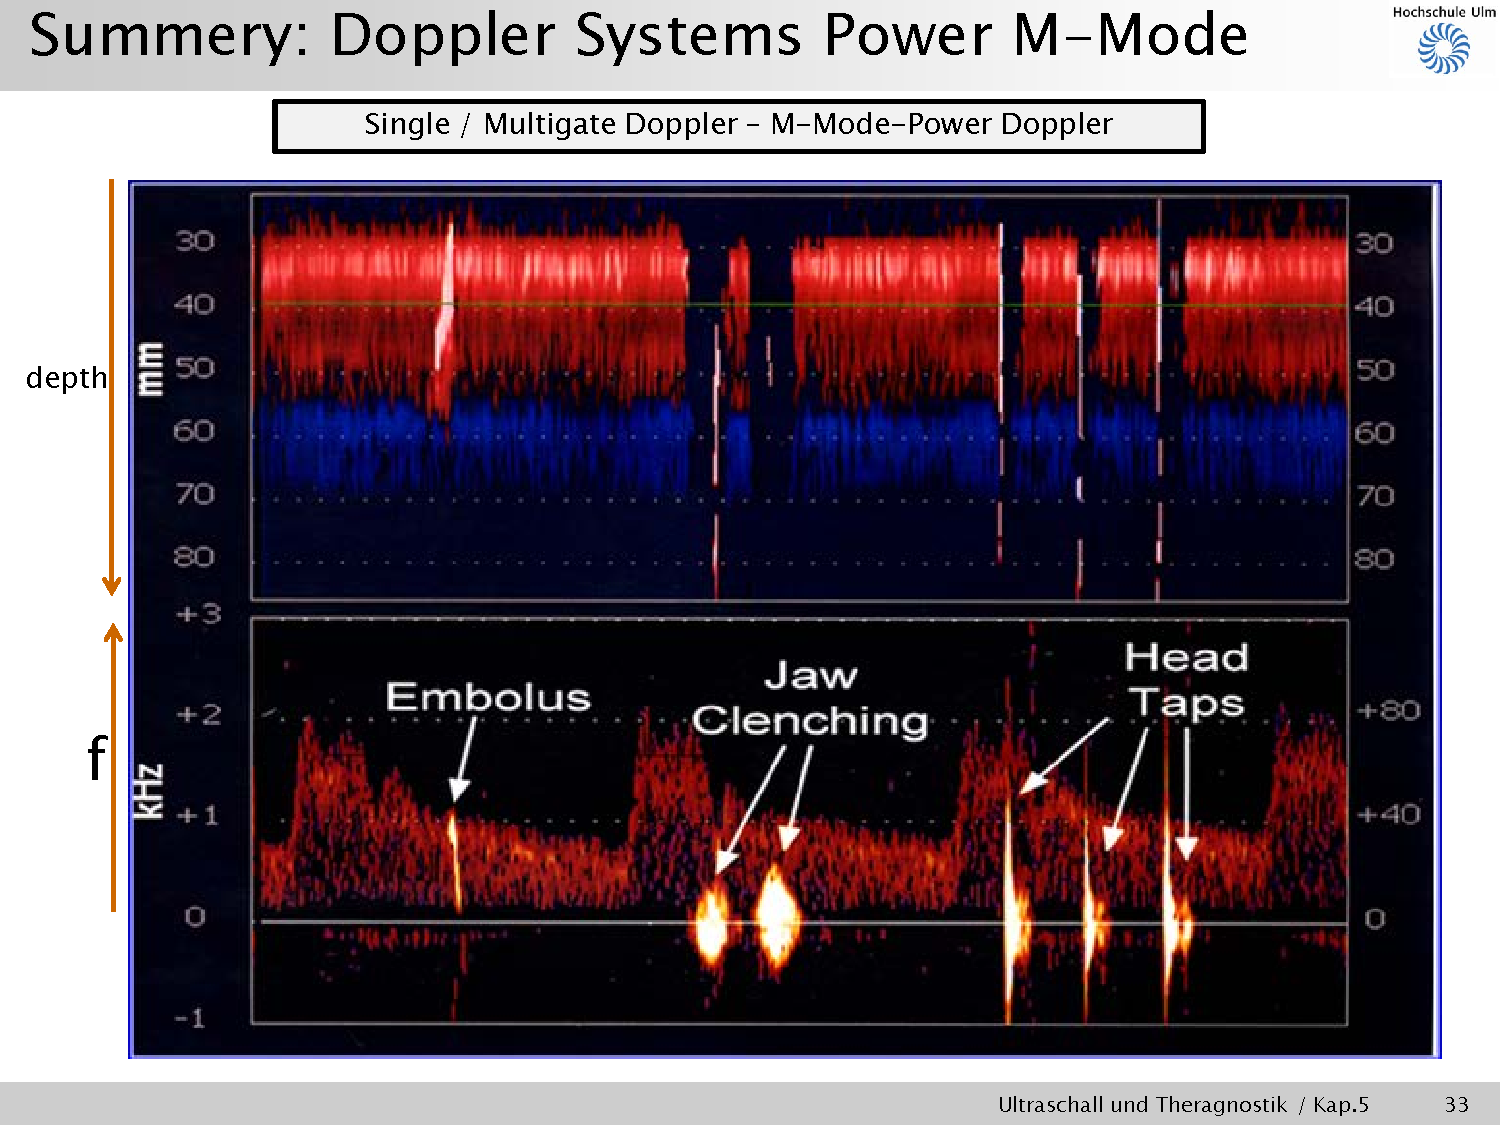
\includegraphics[trim = 0.3cm 14mm 1.3cm 3.5cm, clip=true, width=0.8\textwidth]{M-Mode} 
			\caption{M-Mode mir Doppler Spektrogram}
		\end{figure}
\end{frame}
%
%
%
%
\subsection{Probleme und Motivation}
\begin{frame}
	\begin{block}{Probleme}
		\begin{itemize}
			\item geringer Detailgrad pro Kanal
			\item Detailgrad der Hüllkurve bedingt durch Kanalanzahl			
			\item B-/M-Mode durch hohen Hardwareaufwand realisierbar
		\end{itemize}
	\end{block}
	\begin{block}{Motivation}
		\begin{itemize}
			\item Erkennung von Embolien durch Hüllkurve
			\item M-Mode Darstellung für die schnelle Tiefenselektion
			\item Reduzierung der Anschaffungskosten
		\end{itemize}
	\end{block}
\end{frame}



\section{Konzept der Dopplerinstrumentierung}
\subsection{Vergleich konventionelle analoge und Hilbert transformierte Demodulation}
\begin{frame}
\definecolor{fgblue}{rgb}{0,0,0.6}%
\definecolor{fgred}{rgb}{0.6,0,0}%
\begin{figure}[h]
\centering
\begin{tikztimingtable}
[auto, node distance=3cm,>=latex, scale=0.88, transform shape,
timing/d/background/.style={fill=white},
timing/c/.cd]
Clock 			& 185{0.2C} \\
PRF 			& D{}35D{}D{} \\
BURST 			& [fgblue] L 10{0.1H 0.1L} 33L 5{0.1H 0.1L} \\
ROI CH1	& [fgred] 5L 1{10D{SV}} 22L \\
ROI CH2	& [fgred] 15L 1{10D{SV}} 12L \\
ROI CH3	& [fgred] 25L 1{10D{SV}} 2L \\
ADC				& [fgblue] 5L 30H 2L \\
ROI		& [fgblue] 5L 15{2D{SV}} 2L \\
Retransmit		& L G 35L G L \\
\extracode
	\draw (0 ,0) circle (0.5 pt); % Origin
	\begin{pgfonlayer}{background}
		\vertlines [help lines]{1,3,5,15,25,35,36}
	\end{pgfonlayer}
%	\tablegrid
\end{tikztimingtable}
\caption{Ereignis-Zeitdiagramm}
\label{fig:pw_timing}
\end{figure}
\end{frame}

\begin{frame}
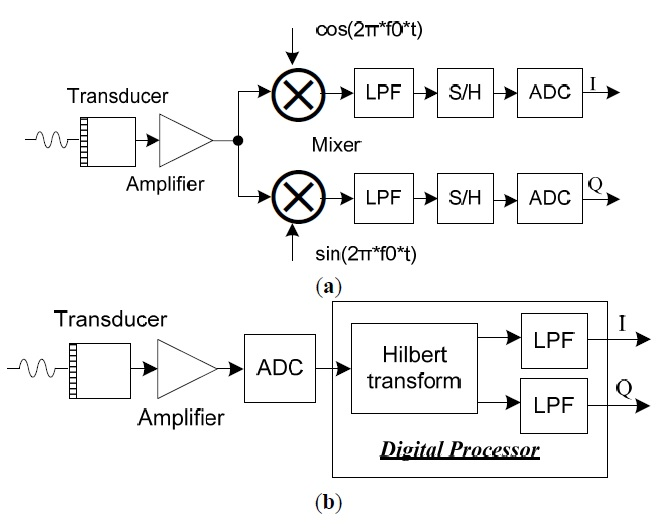
\includegraphics[width=0.9\textwidth]{images/Praesentation/difference}
\end{frame}

\subsection{Signalverarbeitung}
\begin{frame}
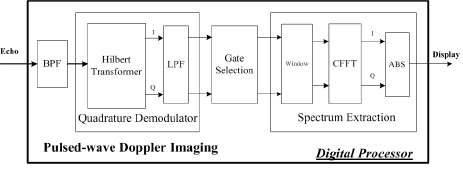
\includegraphics[width=\textwidth]{images/Praesentation/imaging}
\end{frame}

\begin{frame}
	\begin{block}{CPLD / Lattice MachXO2}
		\begin{itemize}
			\item Zustandsautomat mit Peripherieansteuerung
			\item Hilbert transformierte Demodulation + Tiefpassfilter
			\item Zwischenspeicher
		\end{itemize}
	\end{block}
	\begin{block}{ARM Cortex-M4/M0}
		\begin{itemize}
		\item Schnittstelle zwischen PC und CPLD
		\item HS USB 2.0 für die Bewältigung der M-Mode Datenmenge% (theoretisch 60 MB/s)
		\end{itemize}
	\end{block}
\end{frame}


\section{Ergebnisse}
\subsection{Hardware}
\begin{frame}{Platine}
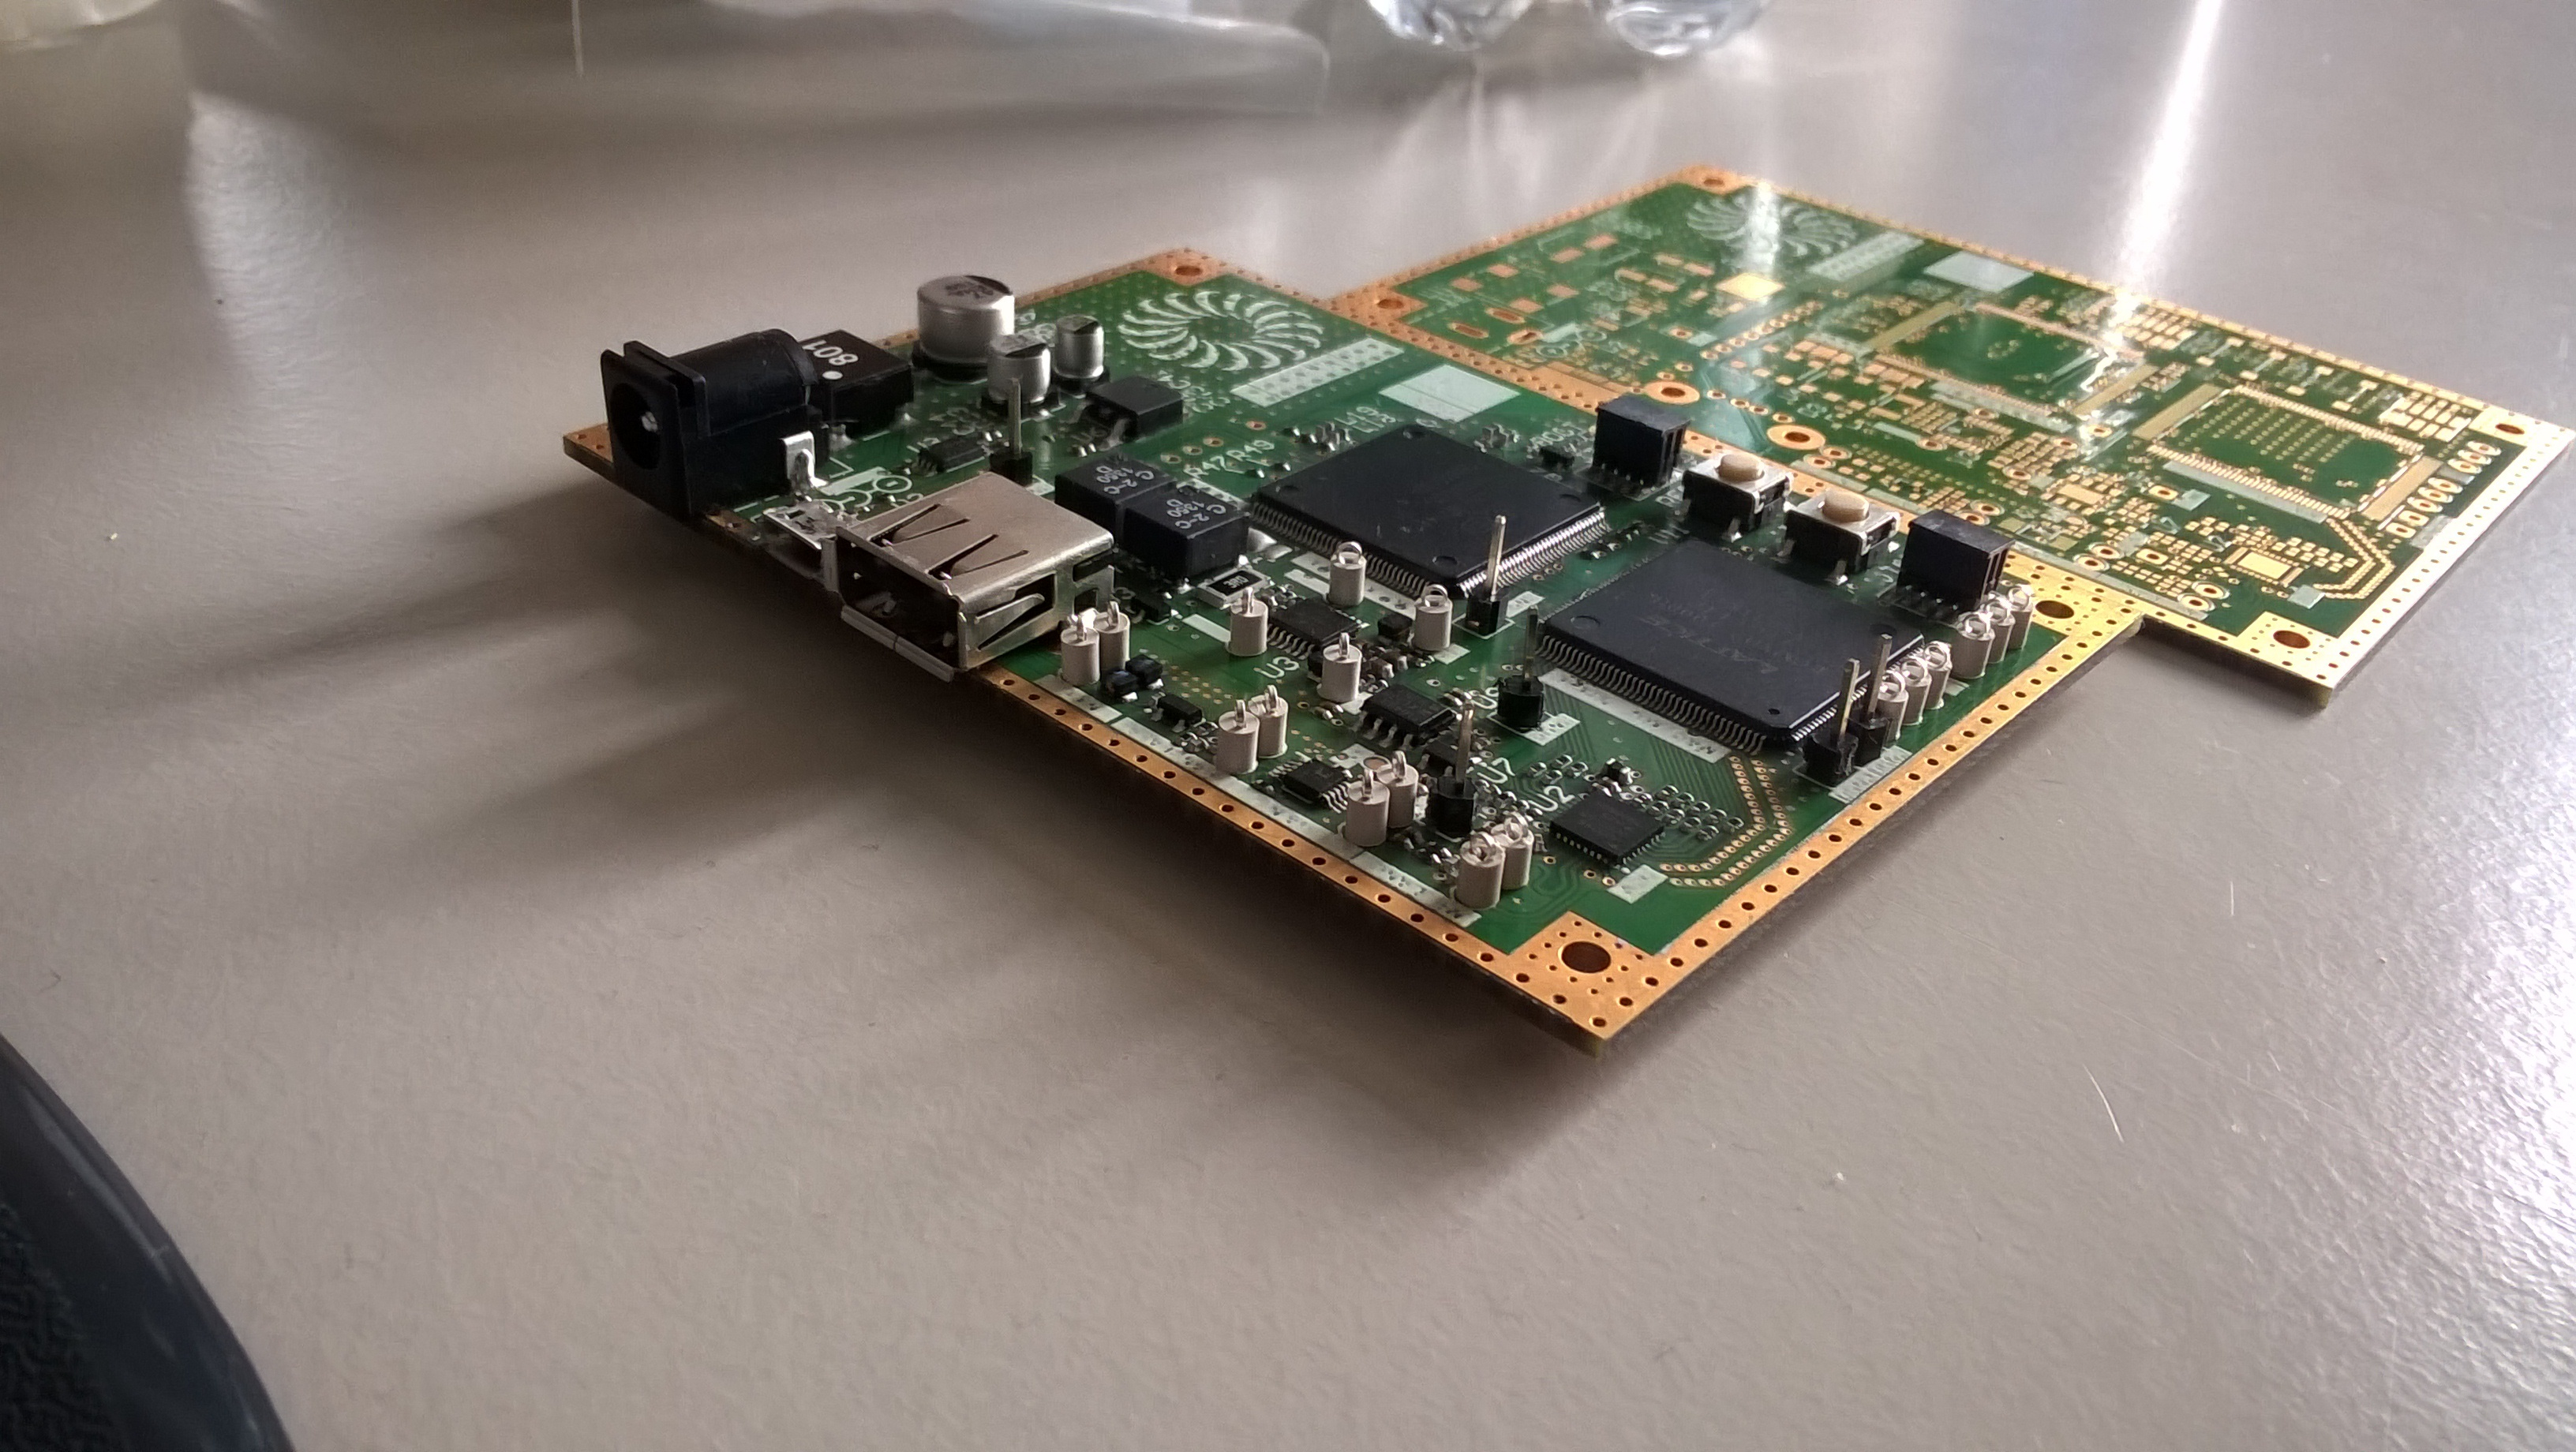
\includegraphics[width=\textwidth, trim= 230mm 155mm 0mm 65mm, clip=true]{images/pcb/WP_20150709_002}
\end{frame}
\begin{frame}{Platinenoberseite}
\begin{figure}[h!]
\centering
\subfloat[Ground Plane]{\includegraphics[page=4,width=0.39\textwidth, trim= 0mm 0mm 0mm 0mm, clip=true]{images/pcb/Job2.PDF}}
\subfloat[animiert]{	\includegraphics[page=3,width=0.43\textwidth, trim= 65mm 0mm 65mm 0mm, clip=true]{images/pcb/Job2.PDF}}
\end{figure}
\end{frame}
%
%
\begin{frame}{Transmitter}
\begin{figure}[h!]
\centering
\subfloat[2 MHz xDSL Signal]{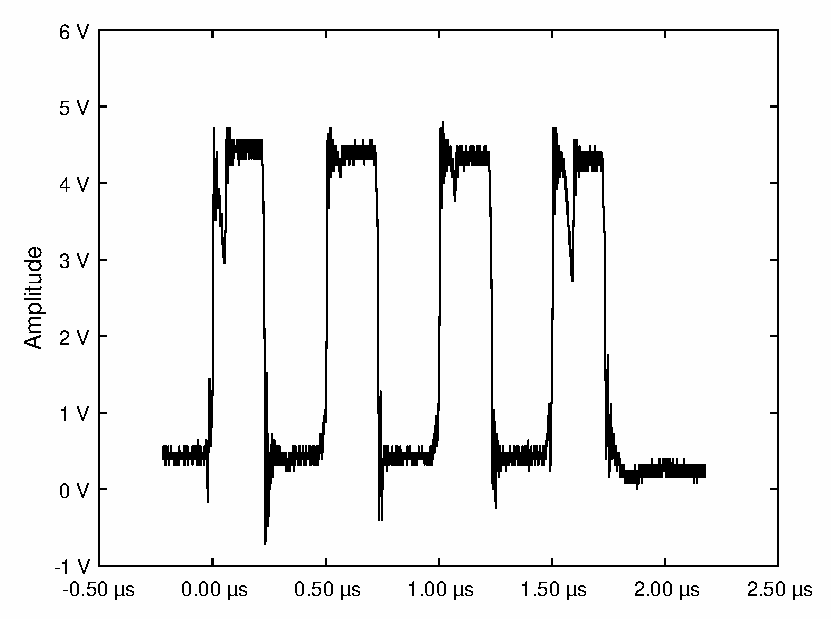
\includegraphics[width=0.3\textwidth, trim= 0mm 0mm 0mm 0mm, clip=true]{images/tests/tx/2MHz-TX.eps}}
\hspace{1mm}
\subfloat[4 MHz xDSL Signal]{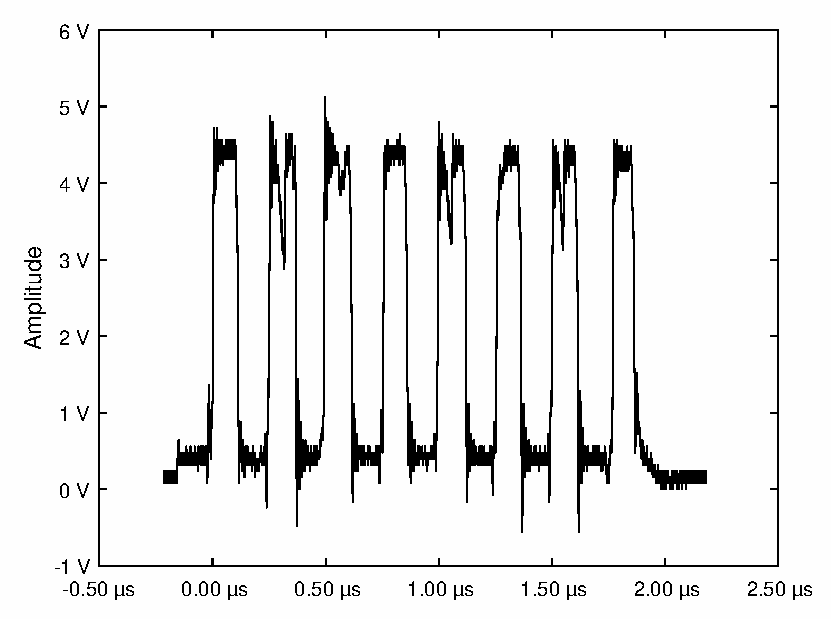
\includegraphics[width=0.3\textwidth, trim= 0mm 0mm 0mm 0mm, clip=true]{images/tests/tx/4MHz-TX.eps}}
\hspace{1mm}
\subfloat[8 MHz xDSL Signal]{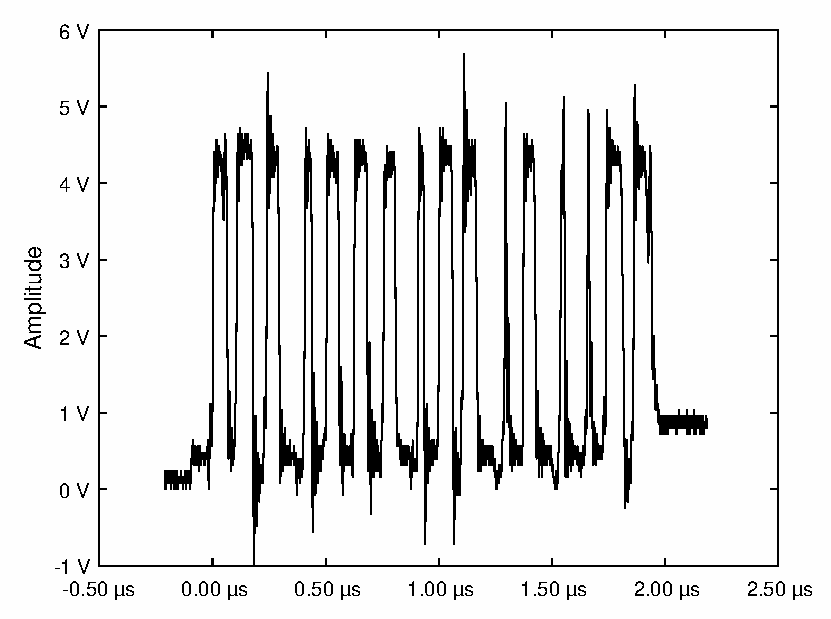
\includegraphics[width=0.3\textwidth, trim= 0mm 0mm 0mm 0mm, clip=true]{images/tests/tx/8MHz-TX.eps}}
\hspace{1mm}
\subfloat[2 MHz Burst]{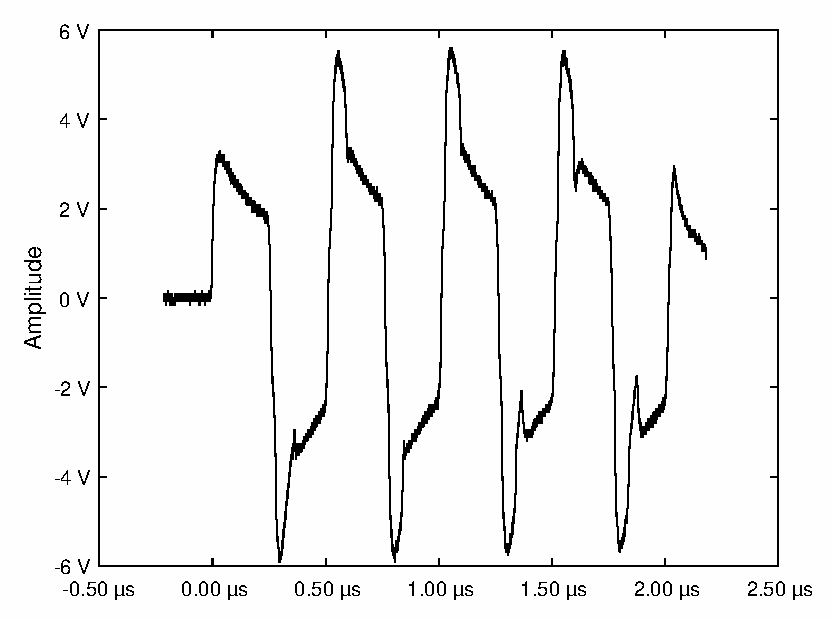
\includegraphics[width=0.3\textwidth, trim= 0mm 0mm 0mm 0mm, clip=true]{images/tests/tx/2MHz-in.eps}}
\hspace{1mm}
\subfloat[4 MHz Burst]{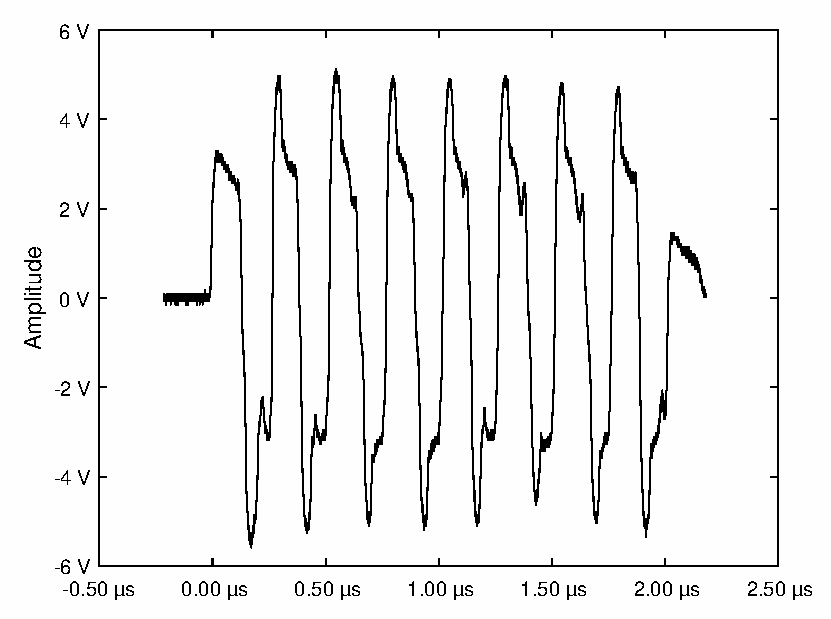
\includegraphics[width=0.3\textwidth, trim= 0mm 0mm 0mm 0mm, clip=true]{images/tests/tx/4MHz-in.eps}}
\hspace{1mm}
\subfloat[8 MHz Burst]{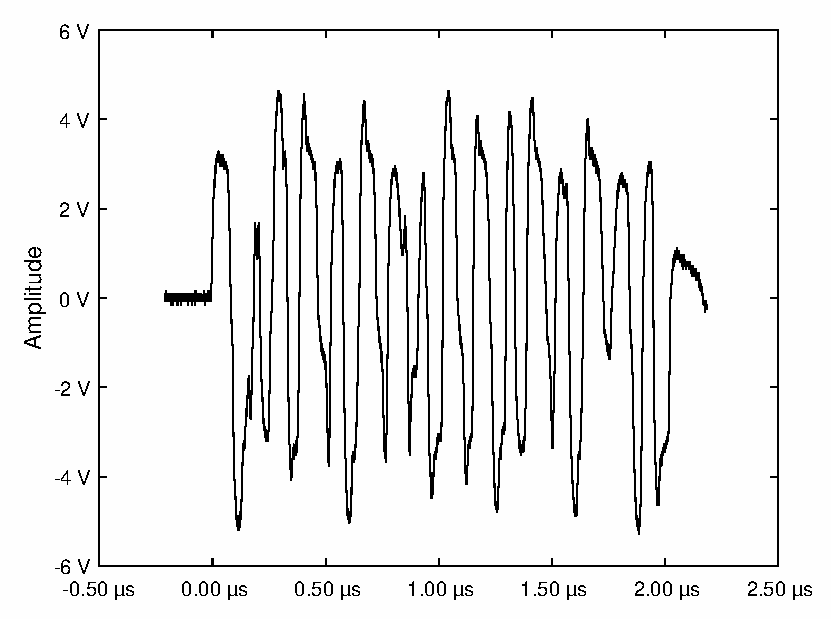
\includegraphics[width=0.3\textwidth, trim= 0mm 0mm 0mm 0mm, clip=true]{images/tests/tx/8MHz-in.eps}}
\end{figure}
\end{frame}
%
%
\begin{frame}{Receiver}
\begin{columns}
\column[b]{.6\textwidth} 
	\begin{center}
    %\setlength{\tabcolsep}{2pt}
    %\small
    \begin{tabular}{r|r|r|c}
			$R_G$ & Faktor & Verstärkung & SNR \\ \hline
8,6 $\Omega$	& 20,00 & 26,0 dB & 59,96 dB \\ 
39 $\Omega$ 	& 9,09	& 19,2 dB & 66,61 dB \\
82 $\Omega$ 	& 5,60	& 14,9 dB & 68,96 dB \\
100 $\Omega$ 	& 4,62	& 13,3 dB & 69,87 dB \\
150 $\Omega$ 	& 3,45	& 10,7 dB & 71,30 dB \\
220 $\Omega$ 	& 2,06	& 6,3  dB & 71,86 dB
\end{tabular}
\captionof{table}{SNR in Abhängigkeit der Verstärkung und Widerstand $R_G$}
  \end{center}%  
	\column[b]{.38\textwidth}
		\begin{figure}[t]
			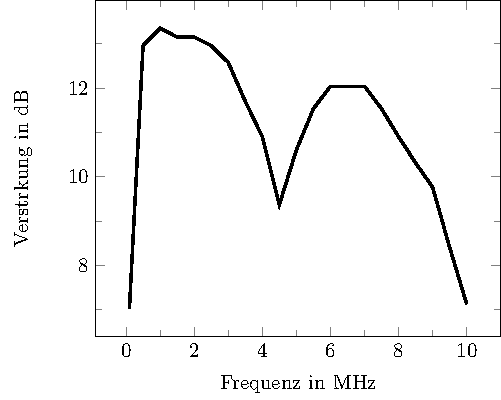
\includegraphics[width=\textwidth, trim= 0mm 0mm 0mm 0mm, clip=true]{images/tests/bandpassDB}
  			\caption{Verstärkung der gesamten Receivermoduls}
		\end{figure}
	\end{columns}
\end{frame}
%
%
\subsection{Logik und Software}
\begin{frame}{Datenübertragung}
\begin{columns}
\column[b]{.4\textwidth} 
	\begin{center}
    \setlength{\tabcolsep}{2pt}
    \small
    \begin{tabular}{l|c|c|l}
\textbf{Port} & \textbf{Hub} & \textbf{Maus} & \textbf{MB/s} \\
\cline{1-4}
USB 3.0 &  	&  	&	38,75	\\ 
USB 3.0 & X	&  	& 38,875	\\
USB 3.0 & X & X & 38,50	\\
\cline{1-4}
USB 2.0 &  	&  	& 34,25	\\
USB 2.0 & X &  	& 34,00	\\
USB 2.0 & X & X	& 32,875
\end{tabular}
\captionof{table}{Datenrate der HS-USB Schnittstelle des LPC4337}
  \end{center}%  
	\column[b]{.58\textwidth}
		\begin{figure}[t]
			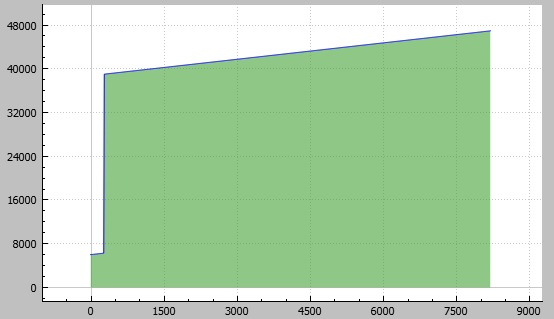
\includegraphics[width=\textwidth, trim= 0mm 0mm 0mm 0mm, clip=true]{images/vortrag/transfer-Counter1}
  			\caption{Datenübertragung von Zählwerten ohne FIFO}
		\end{figure}
	\end{columns}
\end{frame}
%
%
\begin{frame}{GUI}
  \begin{figure}[t]
	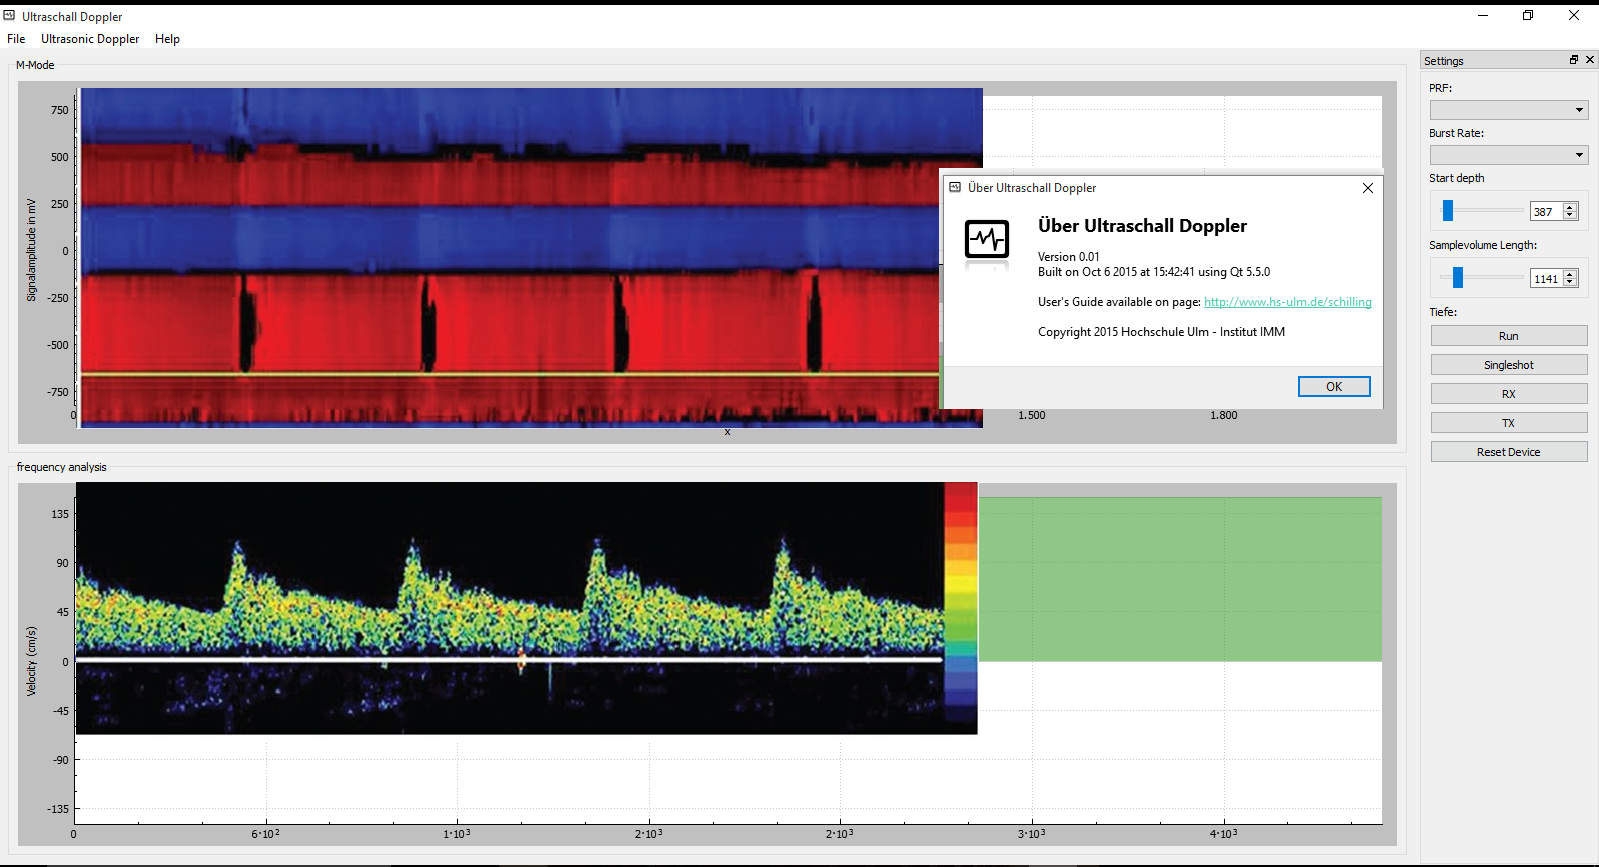
\includegraphics[width=0.9\textwidth, trim= 0mm 0mm 0mm 0mm, clip=true]{images/software/Programm}
  	\caption{Programm}
  \end{figure}
\end{frame}

\begin{frame}{Visualisierung}
  \begin{figure}[h!]
  \centering
	\subfloat[single burst]{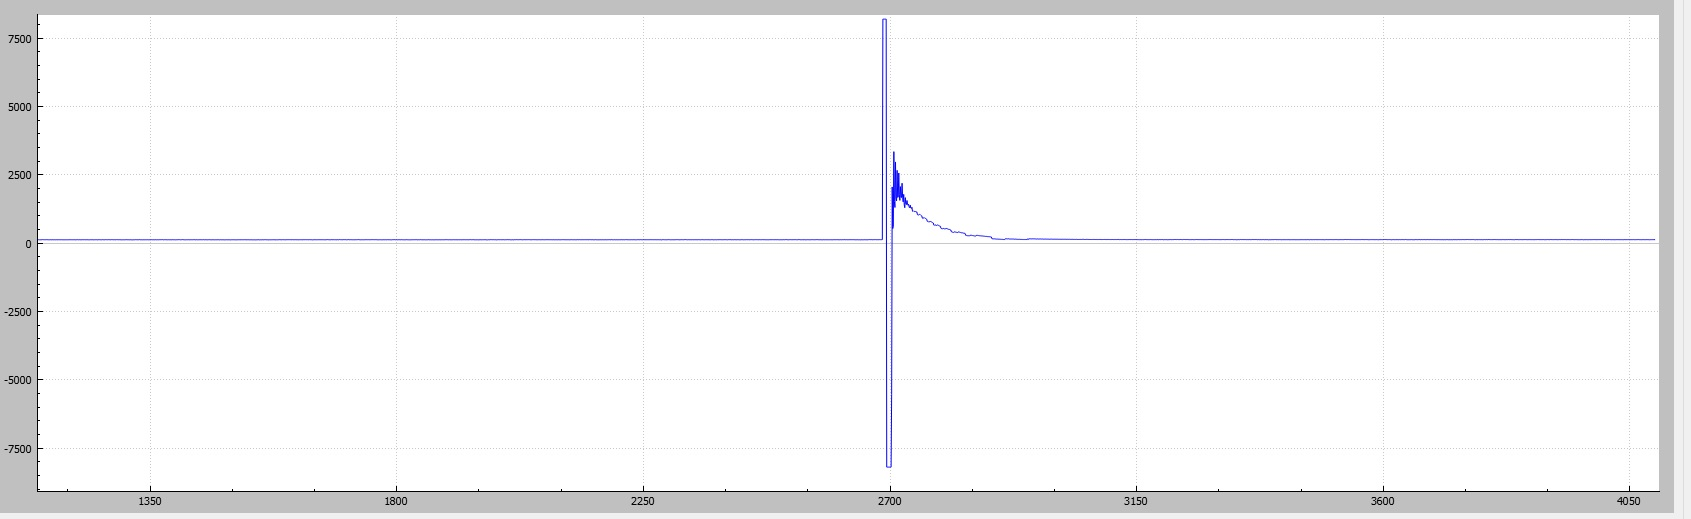
\includegraphics[width=0.6\textwidth, trim= 40mm 0mm 20mm 0mm, clip=true]{images/vortrag/burst_measurement}}
	\hspace{1mm}
	%\subfloat[single burst]{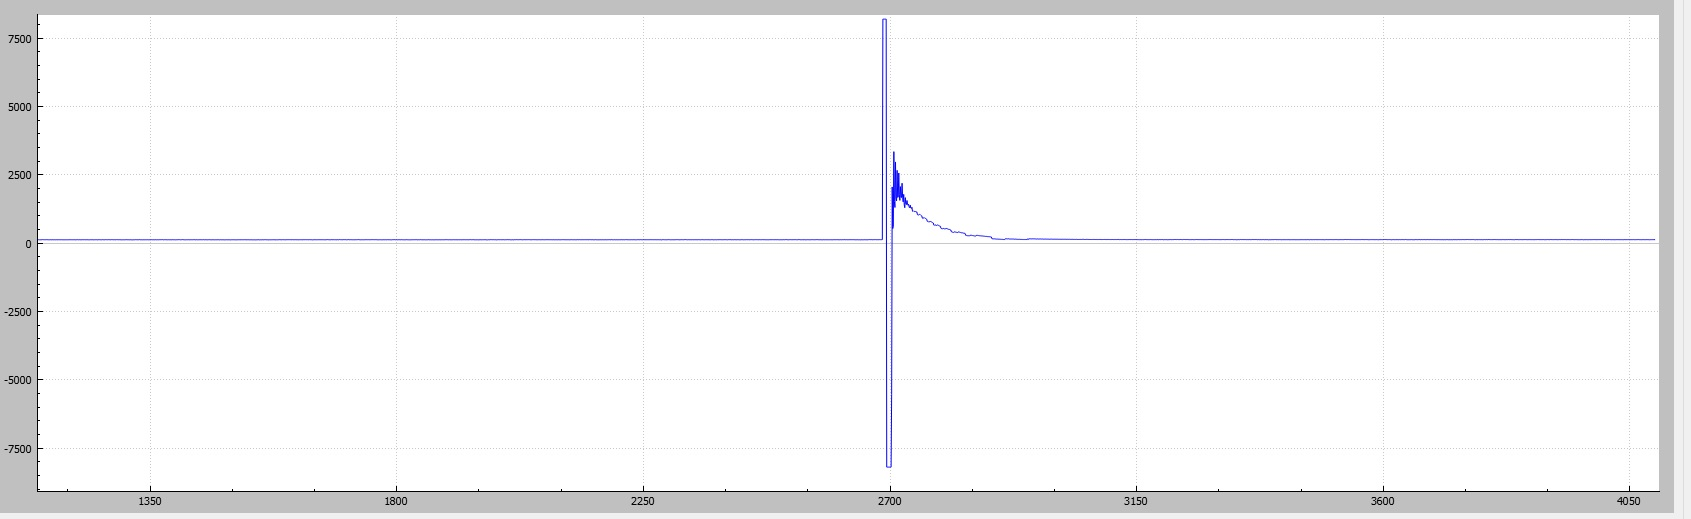
\includegraphics[width=0.2\textwidth, trim= 210mm 0mm 170mm 0mm, clip=true]{images/vortrag/burst_measurement}}
	%\hspace{1mm}
	\subfloat[sporadischer Byteshift bei leerem FIFO]{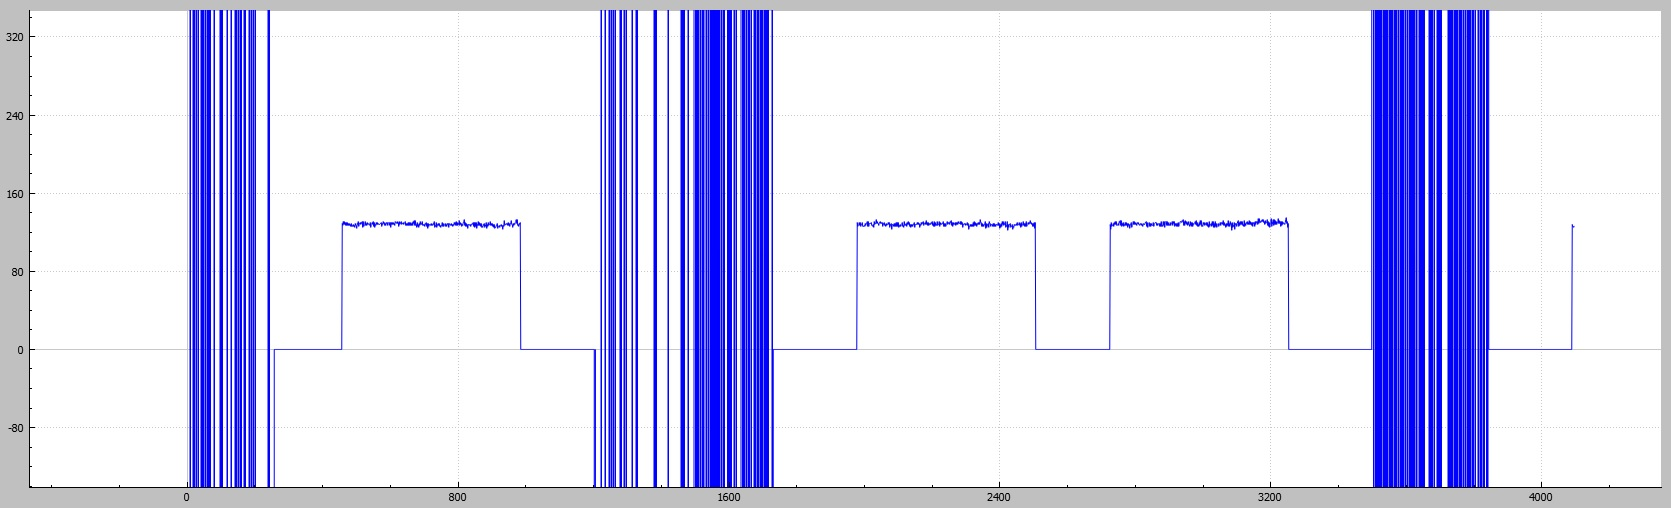
\includegraphics[width=0.6\textwidth, trim= 40mm 0mm 20mm 0mm, clip=true]{images/vortrag/noise_measurement}}
  \end{figure}
\end{frame}

\section{Potenzial und Ausblick}
\subsection*{Potenzial und Ausblick}
\begin{frame}
	\begin{block}{Potenzial}
	\begin{itemize}
		\item M-Mode kann durch hohe Datenrate visualisiert werden
		\item Erkennung von Embolien möglich
%		\item Kosten-/ Platzreduzierung
		\item Grundlage für weitere Entwicklungen möglich 
	\end{itemize}	
	\end{block}
	\begin{block}{Ausblick}
	\begin{itemize}
		\item Transmitter separat betrachten und Konzept überdenken
		\item Receiver - SNR Optimierung durch Layoutüberarbeitung %\tick \fail
		\item simulierte Demodulierung implementieren
		\item Datenstream zwischen PC und Instrumentierung synchronisieren
	\end{itemize}
	\end{block}
\end{frame}

\subsection*{}
\begin{frame}
Danke für Ihre Aufmerksamkeit!
\end{frame}

\end{document}
